\documentclass[11pt]{article}
\usepackage[utf8]{inputenc}
\usepackage{setspace}
\usepackage[top=20mm, bottom=20mm, left=25mm, right=25mm,
  headheight=12pt, headsep=4mm, footskip=8mm]{geometry}
\usepackage{indentfirst}
\usepackage{graphicx}
\usepackage{wrapfig}
\usepackage{caption}
\usepackage{subcaption}
\usepackage{float}
\usepackage{placeins}
\usepackage{color}
\usepackage{amsmath,amsthm,amssymb}
\usepackage{kpfonts}
\usepackage{booktabs}

\setlength{\parindent}{0pt}
\setlength{\parskip}{0.65\baselineskip plus 2pt minus 1pt}

\captionsetup{margin=10pt,font=small,labelfont=bf}

\newcommand{\reporttitle}{Simulation Methods for Finance}
\newcommand{\subtitle}{Part 2 Review: Multilevel Monte Carlo Path Simulation\\
Michael B.\ Giles, \textit{Operations Research} 56(3), 2008}
\newcommand{\reportauthor}{
Anran Severac (CID: 06059786)\\
Ash Sharma (CID: 06049199)\\
Dev Singhrai (CID: 06052090)\\
}
\newcommand{\reporttype}{Coursework}

%%%%%%%%%%%%%%%%%%%%%%%%%%%%

\begin{document}
\begin{titlepage}
\centering
\vspace*{2cm}

{\Large\textsc{Imperial College London}}\\[0.3cm]
{\large Department of Mathematics}\\[2cm]

{\LARGE\textbf{MATH70113}}\\[0.3cm]
{\Large\reporttitle}\\[0.8cm]
{\large\reporttype}\\[1.5cm]

\rule{0.8\textwidth}{0.4pt}\\[0.8cm]
{\large\subtitle}\\[0.8cm]
\rule{0.8\textwidth}{0.4pt}\\[2cm]

{\large\reportauthor}\\[2cm]

{\large March 2026}

\vfill
\end{titlepage}


%=============================================================================
\section{Introduction}
%=============================================================================

Monte Carlo simulation is the dominant numerical method for pricing path-dependent derivatives whose payoff structures preclude closed-form solutions. However, the cost of a na\"ive Monte Carlo estimator grows sharply with the accuracy requirement: achieving root-mean-square (RMS) error $\varepsilon$ with a first-order weak discretisation demands $O(\varepsilon^{-2})$ independent paths, each requiring $O(\varepsilon^{-1})$ timesteps, yielding total complexity $O(\varepsilon^{-3})$. This cubic scaling becomes prohibitive for tight accuracy targets and motivates the development of variance reduction techniques that can break the cost--accuracy bottleneck.

Giles~\cite{giles2008} introduces a multilevel Monte Carlo (MLMC) method that exploits a hierarchy of discretisation levels to achieve dramatically lower computational cost. The central insight is a telescoping decomposition: rather than estimating the expected payoff on a single fine grid, the estimator expresses it as a sum of corrections between successive refinement levels. Because each correction is computed from a coupled pair of paths sharing the same Brownian motion, its variance is small, and the number of samples required at each level can be tuned independently. The resulting complexity drops to $O(\varepsilon^{-2}(\log\varepsilon)^{2})$ under Euler--Maruyama discretisation, and to $O(\varepsilon^{-2})$ when the Milstein scheme is used instead.

In this report we review the MLMC framework, reproduce its key numerical predictions for a European call under geometric Brownian motion (GBM), and critically evaluate its strengths and limitations. We then introduce the multilevel quasi-Monte Carlo (MLQMC) extension of Giles and Waterhouse~\cite{giles2009}, which replaces standard Monte Carlo sampling on each level with a randomised rank-1 lattice rule, and discuss the conditions under which this combination yields further cost reductions. Finally, we compare both methods in the context of path-dependent exotic options and summarise our findings.

%=============================================================================
\section{Overview of the Method}
%=============================================================================

\subsection{Problem Setting}

We consider a scalar stochastic differential equation (SDE) of the form
\begin{equation}
dS(t) = a(S,t)\,dt + b(S,t)\,dW(t), \quad 0 < t < T,
\label{eq:sde}
\end{equation}
with given initial data $S_0$. The quantity of interest is the expected value $\mathbb{E}[P]$ of a (possibly path-dependent) payoff functional $P = f(S(t),\, 0 \le t \le T)$. For a European call the payoff depends only on the terminal value, $P = e^{-rT}(S(T) - K)^{+}$, but the framework applies equally to Asian, lookback, barrier, and digital options.

A numerical discretisation with timestep $h$ produces an approximate payoff $\hat{P}$. Standard weak-convergence theory guarantees that the bias $|\mathbb{E}[\hat{P} - P]| = O(h)$ for first-order schemes such as Euler--Maruyama. To make this bias at most $\varepsilon$ one sets $h = O(\varepsilon)$, requiring $O(\varepsilon^{-1})$ timesteps per path. The variance of the Monte Carlo estimator based on $N$ independent paths is $\mathrm{Var}[\hat{P}]/N$; making this at most $\varepsilon^{2}$ requires $N = O(\varepsilon^{-2})$ paths. The total cost is therefore $N \times h^{-1} = O(\varepsilon^{-3})$.

\subsection{The Multilevel Telescoping Identity}

Let $h_{l} = M^{-l}T$ for $l = 0, 1, \ldots, L$, with refinement factor $M$ (typically $M = 2$ or $M = 4$), and let $\hat{P}_{l}$ denote the payoff approximation at level~$l$. Because expectation is a linear operator,
\begin{equation}
\mathbb{E}[\hat{P}_{L}]
= \mathbb{E}[\hat{P}_{0}]
+ \sum_{l=1}^{L}\mathbb{E}\!\bigl[\hat{P}_{l} - \hat{P}_{l-1}\bigr].
\label{eq:telescoping}
\end{equation}
This expresses the fine-level expectation as a coarsest-level estimate plus a sequence of corrections. Each correction $\hat{P}_{l} - \hat{P}_{l-1}$ is estimated independently, using $N_{l}$ samples. The key to the method's efficiency is that the fine and coarse payoffs within each correction are computed from the \emph{same} underlying Brownian path: the fine path uses timestep $h_{l}$, while the coarse path is constructed by summing groups of $M$ consecutive fine-level Brownian increments. This coupling ensures that $\hat{P}_{l}$ and $\hat{P}_{l-1}$ are close pathwise, so the variance $V_{l} = \mathrm{Var}[\hat{P}_{l} - \hat{P}_{l-1}]$ is much smaller than $\mathrm{Var}[\hat{P}_{l}]$.

\subsection{Optimal Sample Allocation}

The variance of the combined estimator $\hat{Y} = \sum_{l=0}^{L}\hat{Y}_{l}$ is $\sum_{l}N_{l}^{-1}V_{l}$, while its computational cost is proportional to $\sum_{l}N_{l}h_{l}^{-1}$. Minimising the variance for a fixed cost (or equivalently minimising cost for a fixed variance) by Lagrange multipliers gives the optimal allocation
\begin{equation}
N_{l} \propto \sqrt{V_{l}\,h_{l}}.
\label{eq:opt_alloc}
\end{equation}
Levels with large variance or large timestep (cheap per-sample) receive more samples; fine levels with small variance receive few. This is the mechanism by which MLMC avoids placing unnecessarily many expensive fine-grid samples.

\subsection{Complexity Theorem}

The main theoretical result of Giles~\cite{giles2008} is summarised in the following theorem. Let $\alpha \ge \tfrac{1}{2}$ denote the weak order and $\beta$ the rate at which the single-sample variance $V_{l}$ decays with~$h_{l}$ (i.e.\ $V_{l} = O(h_{l}^{\beta})$). Then the multilevel estimator can achieve MSE $< \varepsilon^{2}$ with total cost bounded by
\begin{equation}
C \le
\begin{cases}
c\,\varepsilon^{-2}, & \beta > 1,\\[4pt]
c\,\varepsilon^{-2}(\log\varepsilon)^{2}, & \beta = 1,\\[4pt]
c\,\varepsilon^{-2-(1-\beta)/\alpha}, & 0 < \beta < 1.
\end{cases}
\label{eq:complexity}
\end{equation}
For the Euler--Maruyama scheme applied to a European call with Lipschitz payoff, $\alpha = 1$ and $\beta = 1$, yielding $O(\varepsilon^{-2}(\log\varepsilon)^{2})$. The Milstein scheme improves strong convergence to first order, giving $\beta = 2$ and hence the optimal $O(\varepsilon^{-2})$ rate for a broader class of options~\cite{giles2008b}.

%=============================================================================
\section{Strengths and Weaknesses}\label{sec:strengths_weaknesses}
%=============================================================================

\subsection{Strengths}

\textbf{Variance reduction through path coupling:}
The defining feature of MLMC is that the correction estimators $\hat{P}_{l} - \hat{P}_{l-1}$ have much lower variance than $\hat{P}_{l}$ itself. Our numerical experiments confirm that this variance decays as $O(h_{l})$ for the Euler scheme applied to a Lipschitz payoff, which is the rate predicted by theory. This is not merely a constant-factor improvement: it fundamentally changes the cost--accuracy scaling from $O(\varepsilon^{-3})$ to $O(\varepsilon^{-2}(\log\varepsilon)^{2})$, and in the Milstein case to $O(\varepsilon^{-2})$. The practical consequence is that fine-grid simulations, which dominate the cost of standard MC, are needed for only a small fraction of the total sample budget.

\textbf{Model-agnostic hierarchy:}
The multilevel framework does not depend on the specific form of the SDE or the payoff, provided one can construct a consistent coupling between coarse and fine paths. This makes the approach broadly applicable: Giles~\cite{giles2008} demonstrates it for European, Asian, lookback, barrier, and digital options, and subsequent work has extended it to jump-diffusion models~\cite{xia2012}, stochastic volatility~\cite{giles2015}, and PDE-based approaches~\cite{cliffe2011}. The same telescoping structure can be reused with minimal modification whenever a new discretisation or payoff is introduced.

\textbf{Adaptive diagnostics:}
Unlike black-box variance reduction methods, MLMC provides observable per-level quantities (sample variance $V_{l}$, sample mean $\hat{Y}_{l}$, and cost $C_{l}$) that allow the algorithm to allocate samples optimally at runtime and to determine when the bias is sufficiently small. This transparency makes the method practical and auditable: a practitioner can verify that the variance decay rate matches theoretical expectations and detect problems (e.g.\ non-Lipschitz payoffs degrading the rate) before trusting the final estimate.

\subsection{Weaknesses}

\textbf{Sampling inefficiency on each level:}
Although MLMC reduces the total number of samples needed across levels, the sampling engine on each individual level is still standard Monte Carlo with i.i.d.\ draws. The integration error in sample size therefore remains $O(N^{-1/2})$ on every level. Once the discretisation hierarchy has been optimised, this per-level MC rate becomes the residual bottleneck. In high-accuracy regimes, the $\varepsilon^{-2}$ dependence on sample count (even with the multilevel allocation) still implies substantial computational effort.

\textbf{Slow convergence to the expected value:}
Relatedly, to achieve RMS error $\varepsilon$, the total number of paths across all levels scales at least as $\varepsilon^{-2}$. For applications requiring very tight tolerances (e.g.\ regulatory capital calculations or counterparty credit valuation adjustments), the absolute number of paths can still be very large, even if the per-path cost is efficiently distributed.

\textbf{Synthetic benchmarks only:}
The numerical evidence in Giles~\cite{giles2008} is based entirely on GBM with constant coefficients. While this is the standard test case for establishing rates, it does not address the additional complications that arise in practice: calibrated local or stochastic volatility surfaces, multi-asset correlation structures, or real market data with jumps and microstructure effects. The theoretical rates depend on regularity assumptions (e.g.\ uniform Lipschitz bounds on the payoff and diffusion coefficients) that may not hold exactly in production settings.

%=============================================================================
\section{Numerical Experiments}\label{sec:experiments}
%=============================================================================

We reproduce the canonical numerical experiments from Giles~\cite{giles2008} for a European call under GBM: $dS = rS\,dt + \sigma S\,dW$ with $S(0) = 1$, $K = 1$, $r = 0.05$, $\sigma = 0.2$, $T = 1$. The Euler--Maruyama discretisation is used with refinement factor $M = 4$. All code is contained in the accompanying Jupyter notebook \texttt{mlmc\_giles2008.ipynb}.

\subsection{Variance and Bias Decay}\label{subsec:var_bias}

Figure~\ref{fig:var_bias} (left) plots $\log_{M}\mathrm{Var}[\hat{P}_{l}]$ and $\log_{M}\mathrm{Var}[\hat{P}_{l} - \hat{P}_{l-1}]$ against level~$l$ for $l = 0,\ldots,6$, each estimated from 5{,}000 samples. The variance of the payoff itself, $\mathrm{Var}[\hat{P}_{l}]$, remains roughly constant across levels, reflecting the fact that the option's intrinsic randomness does not vanish with refinement. In contrast, the variance of the coupled correction $\hat{P}_{l} - \hat{P}_{l-1}$ declines at approximately slope $-1$ in $\log_{M}$ scale, confirming the theoretically expected $V_{l} = O(h_{l})$ rate for Euler discretisation of a Lipschitz payoff.

Figure~\ref{fig:var_bias} (right) shows the absolute level means $|\mathbb{E}[\hat{P}_{l} - \hat{P}_{l-1}]|$ on a logarithmic scale, together with the timestep $h_{l}$ for reference. The level means decay at a rate consistent with $O(h_{l})$, confirming first-order weak convergence and providing the data-driven stopping criterion used in the algorithm: once $|\hat{Y}_{L}|$ is sufficiently small relative to the target accuracy, the bias is controlled and no further levels are needed.

\begin{figure}[H]
\centering
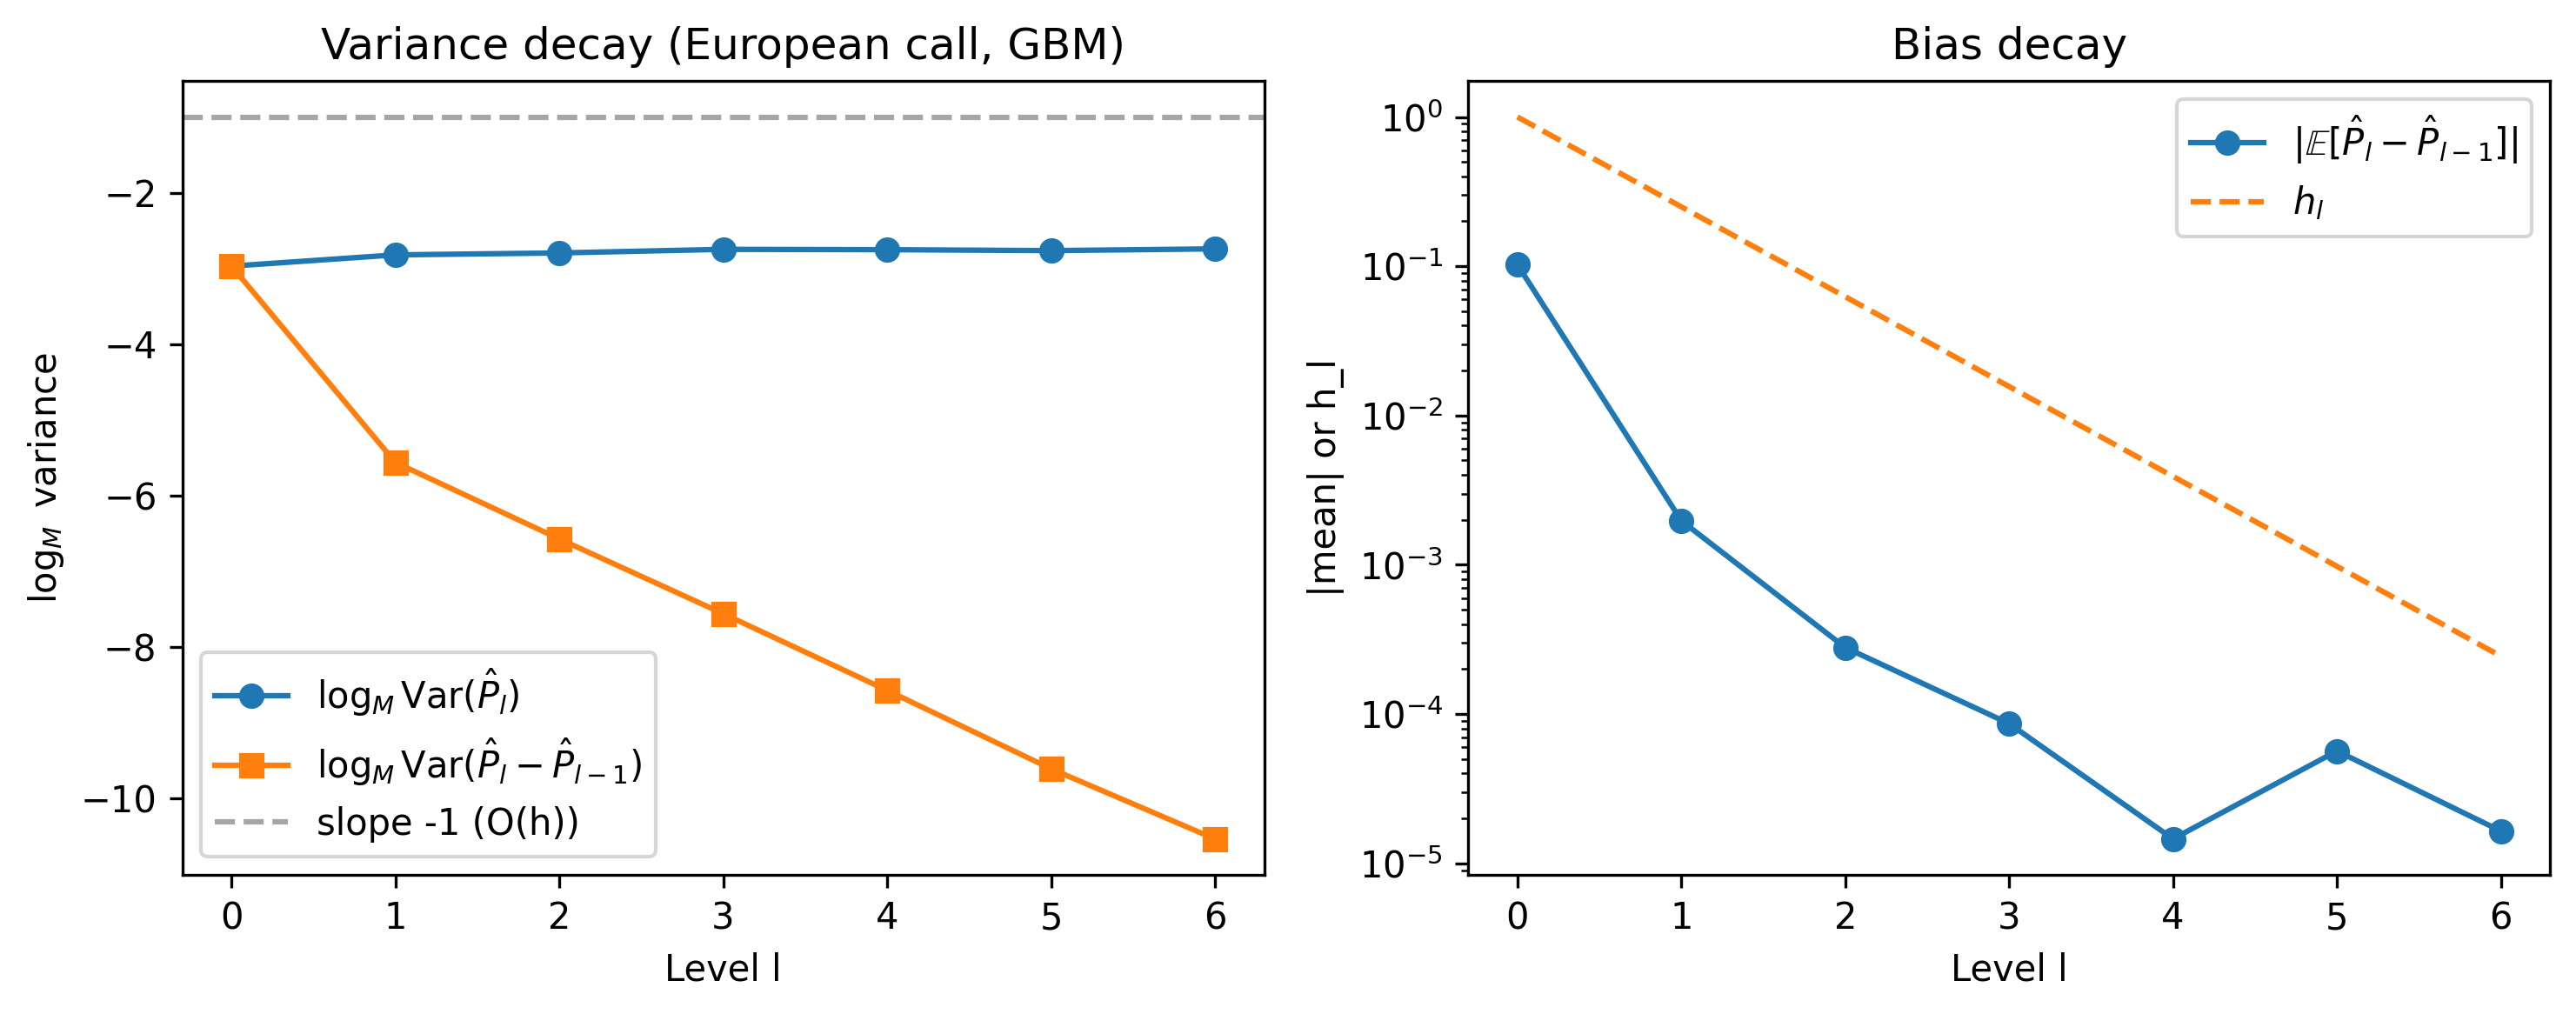
\includegraphics[width=\textwidth]{Images/var_bias_decay.png}
\caption{Variance decay (left) and bias decay (right) across MLMC levels for a European call under GBM with Euler discretisation and $M=4$. The variance of the coupled correction $\hat{P}_{l} - \hat{P}_{l-1}$ decays like $O(h_{l})$ (slope $-1$), while the payoff variance $\mathrm{Var}[\hat{P}_{l}]$ remains roughly constant.}
\label{fig:var_bias}
\end{figure}

\subsection{Computational Cost Scaling}\label{subsec:cost}

Figure~\ref{fig:cost} plots $\varepsilon^{2} \times C$ against $\varepsilon$ for both MLMC and standard Monte Carlo, where $C$ is the total number of timesteps across all paths and levels. For standard MC, $\varepsilon^{2} \times C$ grows like $O(\varepsilon^{-1})$ because total cost is $O(\varepsilon^{-3})$. For MLMC, the quantity grows much more slowly, consistent with the theoretical $O((\log\varepsilon)^{2})$ factor. At $\varepsilon = 5 \times 10^{-4}$, MLMC achieves a cost reduction of roughly two orders of magnitude relative to standard MC.

\begin{figure}[H]
\centering
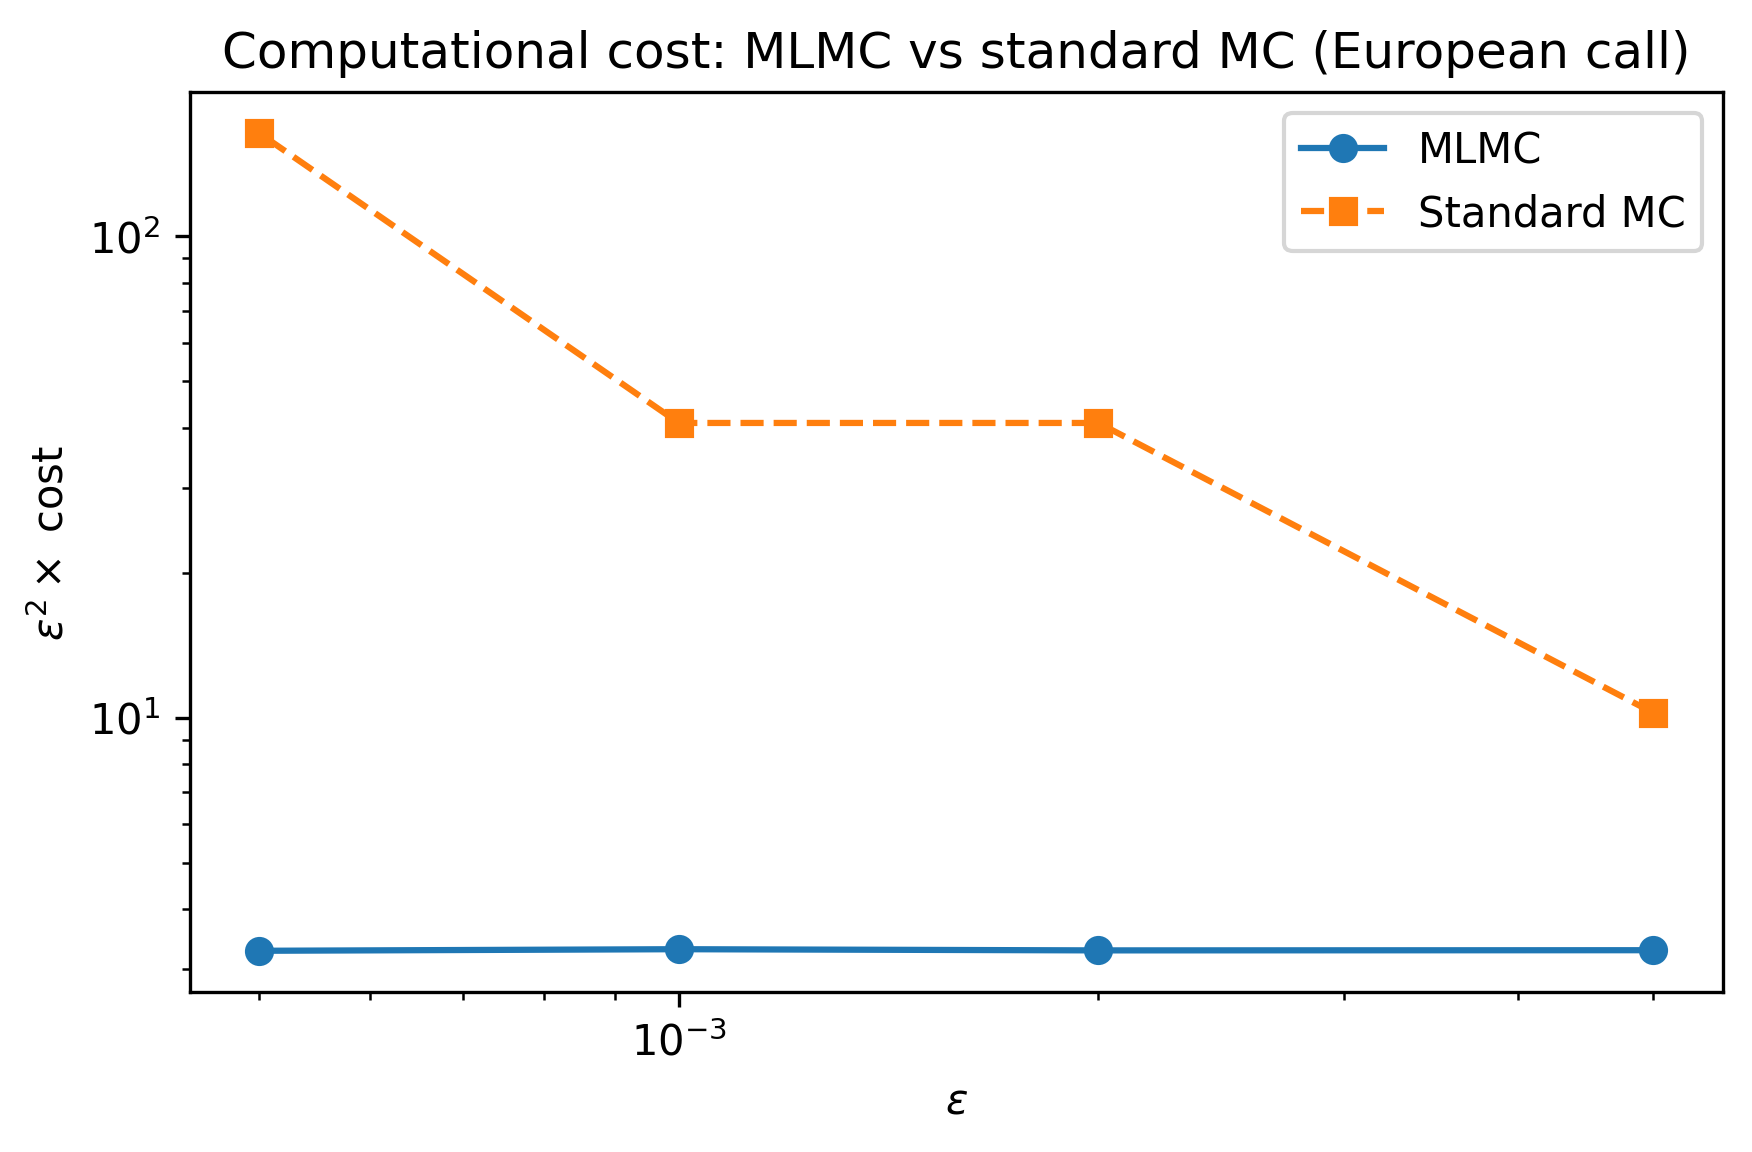
\includegraphics[width=0.65\textwidth]{Images/cost_comparison.png}
\caption{Normalised computational cost $\varepsilon^{2} \times C$ as a function of target accuracy $\varepsilon$, comparing MLMC with standard MC for a European call under GBM.}
\label{fig:cost}
\end{figure}

\subsection{Accuracy Validation}\label{subsec:accuracy}

The Black--Scholes closed-form value for this European call is $V_{\mathrm{BS}} \approx 0.0940$ (computed via the standard formula). The MLMC estimator at target $\varepsilon = 0.001$ returns $\hat{Y} \approx 0.0940$, with the absolute error well within the prescribed tolerance. This validates both the implementation and the bias-control mechanism.

\subsection{Heston Robustness Check}\label{subsec:heston_check}

To extend the baseline GBM experiment, we also simulate a European call under the Heston stochastic volatility model using Euler full-truncation dynamics for variance. We keep a comparable one-year at-the-money setup ($S_0 = K = 1$, $T=1$, $r=0.05$), with reasonable stochastic-volatility parameters
\[
v_0 = 0.04,\quad \kappa = 2.0,\quad \theta = 0.04,\quad \xi = 0.5,\quad \rho = -0.5.
\]
These values preserve the same long-run volatility scale as the GBM benchmark (about $20\%$ annualized) while introducing realistic variance mean-reversion and leverage effect.

Fine/coarse MLMC coupling is implemented by generating correlated Brownian increments on the fine grid and aggregating them in blocks of size $M$ to build the coarse path. This keeps the correction structure directly comparable to the GBM implementation in the notebook. Figure~\ref{fig:heston_cost} reports normalized cost scaling for both GBM and Heston, under MLMC and standard Monte Carlo.

\begin{figure}[H]
\centering
\includegraphics[width=0.75\textwidth]{Images/heston_cost_comparison.png}
\caption{Cost scaling comparison under GBM and Heston dynamics. In both models, MLMC remains markedly more efficient than standard Monte Carlo for the same target accuracy.}
\label{fig:heston_cost}
\end{figure}

The key observation is robustness rather than exact slope matching: once volatility becomes stochastic, variance convergence is less regular than in GBM, but MLMC still provides substantial computational gains over single-level Monte Carlo. This supports the claim that the multilevel construction remains useful beyond the constant-volatility testbed.

\FloatBarrier

%=============================================================================
\section{Extension: Multilevel Quasi-Monte Carlo}\label{sec:qmc}
%=============================================================================

\subsection{Motivation}

The per-level sampling inefficiency identified in Section~\ref{sec:strengths_weaknesses} motivates a natural upgrade: replace i.i.d.\ Monte Carlo sampling with quasi-Monte Carlo (QMC) integration, which can achieve faster convergence for sufficiently smooth integrands. Giles and Waterhouse~\cite{giles2009} pursue exactly this strategy, combining the multilevel hierarchy with a randomised rank-1 lattice rule.

\subsection{Quasi-Monte Carlo Integration}

QMC methods approximate an integral over the unit hypercube $[0,1]^{d}$ using a deterministic set of $N$ low-discrepancy points $\{x_{i}\}$:
\begin{equation}
\int_{[0,1]^{d}} f(x)\,dx \approx \frac{1}{N}\sum_{i=0}^{N-1}f(x_{i}).
\label{eq:qmc}
\end{equation}
For a rank-1 lattice rule, the points are constructed as $x_{i} = \{(i/N)\,z\}$, where $z \in \mathbb{Z}^{d}$ is the generating vector and $\{\cdot\}$ denotes the componentwise fractional part. For integrands with sufficient smoothness and an appropriate notion of diminishing importance across dimensions, the integration error can decay as $O(N^{-1+\delta})$ for all $\delta > 0$, compared with $O(N^{-1/2})$ for standard MC~\cite{sloan2004}.

To recover the unbiasedness and confidence intervals of standard MC, Giles and Waterhouse~\cite{giles2009} use \emph{randomisation}: a uniformly distributed random offset $\Delta \in [0,1)^{d}$ is added to each lattice point, $x_{i} = \{(i/N)\,z + \Delta\}$. The average over $N$ points with a single offset is an unbiased estimator; repeating with $q = 32$ independent offsets provides $q$ independent estimates from which confidence intervals can be constructed in the standard way.

\subsection{Brownian Bridge Construction}

The effectiveness of QMC depends on how the uniform dimensions of the hypercube are mapped to the Brownian increments driving the SDE. Three standard approaches are the Cholesky (standard) construction, the Brownian bridge, and principal component analysis (PCA). Giles and Waterhouse~\cite{giles2009} use the Brownian bridge: the first coordinate determines $W(T)$, the second determines $W(T/2)$ conditional on $W(T)$, and so on recursively. This concentrates the most important variation (the overall path level) in the earliest QMC dimensions, which are sampled with the lowest discrepancy, and relegates local path detail to later dimensions. For the option types considered, the Brownian bridge consistently outperforms the standard construction.

\subsection{The Combined MLQMC Algorithm}

At each level~$l$ of the multilevel hierarchy, the standard MC estimator $\hat{Y}_{l}$ is replaced by a QMC estimator using $N_{l}$ lattice points and 32 random offsets. The algorithm proceeds adaptively:
\begin{enumerate}
\item Start with $L = 0$.
\item Estimate the variance $V_{L}$ at the new level using $N_{L} = 1$ lattice point across 32 offsets.
\item While $\sum_{l} V_{l} > \varepsilon^{2}/2$, double $N_{l}$ on the level with the largest ratio $V_{l}/(2^{l}N_{l})$ (maximising variance reduction per unit cost).
\item If $L < 2$ or the bias estimate exceeds $\varepsilon/\sqrt{2}$, set $L := L + 1$ and return to step~2.
\end{enumerate}
This greedy allocation replaces the closed-form $N_{l} \propto \sqrt{V_{l}h_{l}}$ rule because the QMC variance does not scale as $N^{-1}$; instead, doubling $N$ on a given level is the most natural unit of refinement.

\subsection{How MLQMC Addresses the Weaknesses of MLMC}

The QMC component directly targets the sampling-inefficiency weakness identified in Section~\ref{sec:strengths_weaknesses}. On each level, lattice-rule sampling can converge faster than $N^{-1/2}$, particularly on the coarsest levels where the integrand is low-dimensional and relatively smooth. Since the coarsest levels account for the largest share of total cost in the multilevel budget, accelerating convergence there has a disproportionate effect on overall efficiency. The numerical results in Giles and Waterhouse~\cite{giles2009} show that for a European call, the combined MLQMC estimator achieves $\varepsilon^{2} \times C$ roughly constant (i.e.\ cost proportional to $\varepsilon^{-1}$), compared with $\varepsilon^{2} \times C = O((\log\varepsilon)^{2})$ for MLMC alone. This represents an additional factor of 20--100 in cost savings.

On finer levels the QMC advantage diminishes. This is expected: the multilevel corrections on fine levels are high-dimensional (many timesteps) and oscillatory, so the effective smoothness that QMC exploits is reduced. However, because the multilevel hierarchy already ensures that very few samples are placed on fine levels, the loss of QMC efficiency there has little impact on total cost.

\subsection{Limitation: Non-Smooth Payoffs}\label{subsec:nonsmooth}

The theoretical QMC error bounds require smoothness conditions on the integrand that non-smooth payoffs violate. Digital options (discontinuous payoff) and barrier options (indicator function of path minimum) introduce kinks or jumps in the integrand that can degrade the QMC convergence rate toward the Monte Carlo baseline. Giles and Waterhouse~\cite{giles2009} still report empirical gains for these payoff types, but the improvements are less uniform and less dramatic than for smooth payoffs such as European and Asian calls. The MLMC framework from Giles~\cite{giles2008} remains robust in these cases because its complexity bounds depend on strong-convergence rates rather than integrand smoothness.

%=============================================================================
\section{Comparison on Exotic Options}\label{sec:exotic}
%=============================================================================

To place both methods in practical context, we compare MLMC and MLQMC on option types spanning a range of smoothness, drawing on the numerical evidence in both papers as well as our own experiments.

\subsection{Asian Options}

The Asian call payoff $P = e^{-rT}\max(0,\bar{S} - K)$, where $\bar{S} = T^{-1}\int_{0}^{T}S(t)\,dt$, is path-dependent but smooth in the payoff functional. Both Giles~\cite{giles2008} and Giles and Waterhouse~\cite{giles2009} report strong variance decay rates ($\beta \ge 2$ with Milstein) and excellent MLMC performance. Adding QMC further reduces cost by exploiting the smooth dependence of the average on the Brownian path. For this payoff type, MLQMC is unambiguously the method of choice.

\subsection{Lookback Options}

The lookback payoff depends on the path maximum or minimum. The Milstein discretisation with Brownian interpolation~\cite{giles2008b} provides $\beta = 2$ variance decay, and the QMC Brownian bridge construction aligns well with the hierarchical sampling of path extrema. Giles and Waterhouse~\cite{giles2009} report comparable cost reductions to the Asian case.

\subsection{Barrier and Digital Options}

These payoffs introduce discontinuities (the indicator $\mathbf{1}_{\min S > B}$ for barriers, or the step function for digitals). The variance decay rate drops (often to $\beta \approx 1$ even with Milstein for barriers, and $\beta < 1$ for digitals without smoothing), and the QMC integrand is no longer globally smooth. MLMC remains effective because its complexity bound~\eqref{eq:complexity} depends on $\beta$ and $\alpha$ rather than on integrand smoothness per se. MLQMC still offers some improvement, but the gains are problem-specific and cannot be guaranteed by theory. For practitioners working with barrier or digital books, MLMC provides a reliable baseline; MLQMC should be validated empirically on the specific product before being adopted.

\subsection{Summary Comparison}

Table~\ref{tab:comparison} summarises the key differences between the two methods.

\begin{table}[H]
\centering
\small
\setlength{\tabcolsep}{5pt}
\renewcommand{\arraystretch}{1.15}
\begin{tabular}{p{0.30\linewidth} p{0.30\linewidth} p{0.30\linewidth}}
\toprule
\textbf{Aspect} & \textbf{MLMC (Giles 2008)} & \textbf{MLQMC (Giles 2009)} \\
\midrule
Per-level sampling & Standard MC (i.i.d.) & QMC (lattice + randomisation) \\
Convergence in $N$ & $O(N^{-1/2})$ & Up to $O(N^{-1+\delta})$ for smooth integrands \\
Overall cost (Euler, European) & $O(\varepsilon^{-2}(\log\varepsilon)^{2})$ & Empirically ${\sim}\,O(\varepsilon^{-1})$ \\
Non-smooth payoffs & Robust; rate depends on $\beta$ & Gains reduced; theory does not guarantee fast rate \\
Implementation complexity & Straightforward coupling & Requires lattice generation, Brownian bridge, offset management \\
\bottomrule
\end{tabular}
\caption{Comparison of MLMC and MLQMC across key dimensions.}
\label{tab:comparison}
\end{table}

%=============================================================================
\section{Conclusion}
%=============================================================================

The multilevel Monte Carlo method of Giles~\cite{giles2008} represents a fundamental advance in the computational efficiency of Monte Carlo path simulation. By decomposing the fine-grid estimator into a hierarchy of coupled corrections and allocating samples optimally across levels, it reduces complexity from $O(\varepsilon^{-3})$ to $O(\varepsilon^{-2}(\log\varepsilon)^{2})$ under Euler discretisation, and to $O(\varepsilon^{-2})$ with Milstein. Our numerical reproduction confirms the theoretical predictions: correction variances decay at the expected $O(h_{l})$ rate, bias decays consistently with first-order weak convergence, and the $\varepsilon^{2} \times C$ cost metric is substantially lower than for standard Monte Carlo across a range of accuracy targets.

The method's principal strengths are its robustness across payoff types, its model-agnostic structure, and the transparency of its adaptive diagnostics. Its main limitation is the residual $O(N^{-1/2})$ convergence rate on each level, inherited from i.i.d.\ sampling, which Giles and Waterhouse~\cite{giles2009} address by introducing quasi-Monte Carlo integration via randomised lattice rules with Brownian bridge construction. The combined MLQMC estimator achieves further cost reductions of one to two orders of magnitude for smooth payoffs, with cost scaling empirically as $O(\varepsilon^{-1})$. However, QMC gains diminish for non-smooth payoffs (barriers, digitals), where the smoothness assumptions underlying the faster QMC rate are violated.

Together, the two methods form a coherent progression: MLMC provides the foundational architecture that eliminates unnecessary fine-grid sampling through multilevel coupling, and MLQMC adds an integration-level upgrade that accelerates the remaining bottleneck wherever payoff regularity permits. For practitioners, the recommendation is to adopt MLMC as the default framework and to layer QMC on top when payoff smoothness can be verified, either theoretically or through empirical convergence diagnostics.

\begin{thebibliography}{9}

\bibitem{giles2008}
Michael B.\ Giles,
\textit{Multilevel Monte Carlo path simulation},
Operations Research, Vol.~56, No.~3, pp.~607--617, 2008.

\bibitem{giles2008b}
Michael B.\ Giles,
\textit{Improved multilevel Monte Carlo convergence using the Milstein scheme},
in: A.~Keller, S.~Heinrich, H.~Niederreiter (eds.), Monte Carlo and Quasi-Monte Carlo Methods 2006, pp.~343--358, Springer, 2008.

\bibitem{giles2009}
Michael B.\ Giles and Benjamin J.\ Waterhouse,
\textit{Multilevel quasi-Monte Carlo path simulation},
Radon Series on Computational and Applied Mathematics, Vol.~8, pp.~1--18, de~Gruyter, 2009.

\bibitem{sloan2004}
Ian H.\ Sloan, Frances Y.\ Kuo, and Stephen Joe,
\textit{Constructing randomly shifted lattice rules in weighted Sobolev spaces},
SIAM Journal on Numerical Analysis, Vol.~40, No.~5, pp.~1650--1655, 2002.

\bibitem{xia2012}
Yuan Xia and Michael B.\ Giles,
\textit{Multilevel path simulation for jump-diffusion SDEs},
in: Quantitative Finance Papers, Springer, 2012.

\bibitem{giles2015}
Michael B.\ Giles,
\textit{Multilevel Monte Carlo methods},
Acta Numerica, Vol.~24, pp.~259--328, 2015.

\bibitem{cliffe2011}
K.~A.\ Cliffe, Michael B.\ Giles, Robert Scheichl, and Aretha L.\ Teckentrup,
\textit{Multilevel Monte Carlo methods and applications to elliptic PDEs with random coefficients},
Computing and Visualization in Science, Vol.~14, No.~1, pp.~3--15, 2011.

\bibitem{kebaier2005}
Ahmed Kebaier,
\textit{Statistical Romberg extrapolation: a new variance reduction method and applications to option pricing},
Annals of Applied Probability, Vol.~15, No.~4, pp.~2681--2705, 2005.

\end{thebibliography}

\vspace{1.5em}
\noindent\rule{\textwidth}{0.4pt}
\paragraph{Task breakdown.}
\begin{itemize}
\item \textbf{Anran Severac:} MLMC implementation, numerical experiments, MLQMC literature review and discussion.
\item \textbf{Ash Sharma:} Theoretical summary, strengths/weaknesses analysis, exotic option comparison.
\item \textbf{Dev Singhrai:} Report writing, figure generation, accuracy validation.
\end{itemize}

\end{document}
